\chapter{Evaluation}
This section will carry out a critical evaluation of the work undertaken in this paper, and the results of the final
algorithm compared to the targets and metrics set out in the introduction and compared to other works.

\section{Final Results}
The final implementation of the compute shader had two variations:

\begin{itemize}
    \item Monolithic compute shader with colour information encoded in the distance field.
    \item A pure distance field, storing only distance values.
\end{itemize}

The methodology defined that the distance field was to also encode colour information, as seen in
Section~\ref{sec:df_repr}, as such the final testing will be carried out using that version of the compute shader as it
was found that a pure distance field places too much strain of the ray marcher and subsequently heavily affects the FPS
of the application. While the ray marcher wasn't the focus of this paper, achieving a good FPS using the demonstration
application was.

As the final algorithm is a combination of JFA and FIM that is selectively executed depending on whether the chunk being
processed is in the focus area, to determine the single chunk performance of the algorithm a world of $2x2x2$ chunks is
created with the focus area covering points $(0, 0, 0)$ to $(0, 1, 1)$; this will ensure that an even distribution of
updates are JFA only and FIM only. As seen in Table~\ref{tab:final_single_chunk_perf}, we observe that the execution
time of the compute for a single chunk falls below the delta time for a 30 FPS application (33.33ms) for chunk sizes
as high as $256^3$ - in theory this achieves the aim of having a distance field compute shader that can be executed
within a single frame with time left over for other tasks such as rendering at 30 FPS.

While the execution time of the compute shader remains under 33.33ms, the actual FPS of the demonstration application
using $256^3$ chunks is only 1.42 FPS, or only 9.47 FPS for $128^3$ chunk sizes, as seen in
Table~\ref{tab:final_single_chunk_perf}; this does not meet the aim of achieving 30 FPS in the demonstration
application. The ray marcher compute shader, while not the focus of this paper, does impose a significant performance
penalty as seen in Figure~\ref{fig:final_single_chunk_rm}. Combining the execution time of the distance field and ray
marcher compute shader, the FPS of the demonstration application matches what was seen in
Table~\ref{tab:final_single_chunk_perf}.

\begin{table}[h]
    \centering
    \sisetup{
        table-format=3.3,
        round-mode=places,
        round-precision=3
    }
    \vspace{0.5em}
    \resizebox{\textwidth}{!}{%
        \begin{tabular}{l|*{5}{c}}
            \toprule
            \textbf{Chunk Size}          & \textbf{\(16^3\)} & \textbf{\(32^3\)} & \textbf{\(64^3\)} & \textbf{\(128^3\)} & \textbf{\(256^3\)} \\
            \midrule
            \textbf{Avg. Time (ms)}      & 0.022988718       & 0.057287574       & 0.29529586        & 4.571752           & 29.337261          \\
            \textbf{Std. Deviation (ms)} & 0.00283882        & 0.013250402       & 0.036815774       & 1.7831647          & 18.889853          \\
            \textbf{Avg. FPS}            & 163.57758         & 164.06527         & 65.23792          & 9.47038            & 1.42479            \\
            \bottomrule
        \end{tabular}
    }
    \caption{Single chunk performance of an optimized compute shader.}
    \label{tab:final_single_chunk_perf}
\end{table}

\begin{figure}
    \centering
    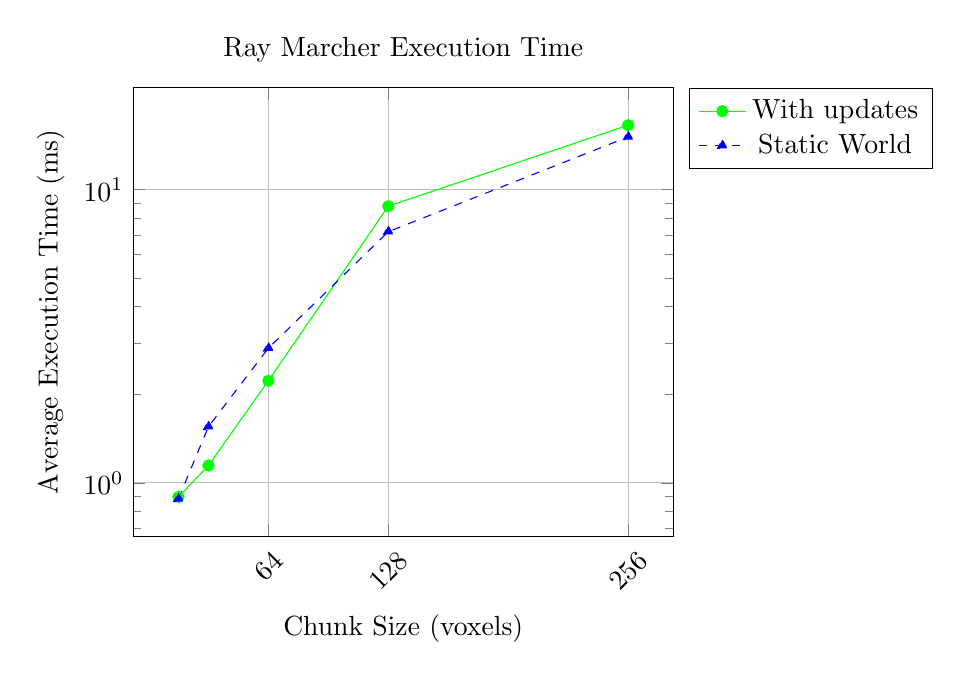
\begin{tikzpicture}
        \begin{axis}[
                title={Ray Marcher Execution Time},
                xlabel={Chunk Size (voxels)}, ylabel={Average Execution Time (ms)},
                xtick={64,128,256,512,1024},
                xticklabel style={rotate=45},
                ymode=log,
                legend pos=outer north east,
                grid=major
            ]

            \addplot[green, solid, mark=*] coordinates {
                    (16,0.8946897) (32,1.1455745) (64,2.2295916) (128,8.784809) (256,16.6005)
                };
            \addlegendentry{With updates}

            \addplot[blue, dashed, mark=triangle*] coordinates {
                    (16,0.8817709) (32,1.5539502) (64,2.8798585) (128,7.191539) (256,15.144967)
                };
            \addlegendentry{Static World}
        \end{axis}
    \end{tikzpicture}
    \caption{Execution time of the ray marching compute shader.}
    \label{fig:final_single_chunk_rm}
\end{figure}

The use of a discrete distance field means every voxel in the world needs to be represented; in the final implementation
each voxel is represented by an ``\textit{uint}'' data type which is 4 bytes. For a world of size $1024^3$ that is a
memory requirement of 4GB to represent the world; this needs to be double as the world is currently represented
twice, once as a distance field, and as a raw voxel grid meaning a total of 8GB is required to represent the world. This
places a hard-limit to the size of the world that can be tested using the hardware available during the testing of this
paper.

We can see in Figure~\ref{fig:final_df_perf} that the distance field execution time of the compute shader at a world
size of $1024^3$ falls below the delta time of a 30 FPS application at all chunk sizes tested, and even below 60 FPS
for chunk sizes equal to or smaller than $128^3$; however, the ray marcher compute shader is a significant bottleneck
and results in a frame rate that does not meet the minimum target of 30 FPS, at any focus size and chunk size
combination.

\begin{figure}
    \centering
    \begin{tikzpicture}
        \begin{groupplot}[
                group style={
                        group size=1 by 3,
                        vertical sep=4cm,
                    },
                grid=major
            ]

            \nextgroupplot[
                title={Distance Field Compute Shader},
                xlabel={Chunk Size (voxels)}, ylabel={Avg. Execution Time (ms)},
                xtick={16,32,64,128,256},
                xticklabel style={rotate=45},
            ]
            \addplot[blue, dotted, mark=*] coordinates {
                    (16,0.07502) (32,0.05740) (64,0.26819) (128,1.86547) (256,21.89112)
                };
            \addlegendentry{$1^3$ Focus Size}
            \addplot[red, thick, mark=*] coordinates {
                    (16,0.07311) (32,0.05764) (64,0.26425) (128,1.90494) (256,25.95815)
                };
            \addlegendentry{$2^3$ Focus Size}
            \addplot[green, dashed, mark=*] coordinates {
                    (16,0.07345) (32,0.05845) (64,0.26478) (128,2.06845) (256,22.34544)
                };
            \addlegendentry{$4^3$ Focus Size}

            \nextgroupplot[
                title={Ray Marcher Compute Shader},
                xlabel={Chunk Size (voxels)}, ylabel={Avg. Execution Time (ms)},
                xtick={16,32,64,128,256},
                xticklabel style={rotate=45},
            ]
            \addplot[blue, dotted, mark=*] coordinates {
                    (16,63.80947) (32,76.99922) (64,46.63217) (128,46.43588) (256,66.91314)
                };
            \addlegendentry{$1^3$ Focus Size}
            \addplot[red, thick, mark=*] coordinates {
                    (16,63.01540) (32,0.05764) (64,57.50888) (128,54.72125) (256,59.43206)
                };
            \addlegendentry{$2^3$ Focus Size}
            \addplot[green, dashed, mark=*] coordinates {
                    (16,65.44576) (32,199.84691) (64,52.55280) (128,47.23503) (256,85.15357)
                };
            \addlegendentry{$4^3$ Focus Size}

            \nextgroupplot[
                title={Frame Performance},
                xlabel={Chunk Size (voxels)}, ylabel={Avg. FPS},
                xtick={16,32,64,128,256},
                xticklabel style={rotate=45},
            ]
            \addplot[blue, dotted, mark=*] coordinates {
                    (16,0.64427) (32,5.67553) (64,13.25291) (128,6.10009) (256,1.15367)
                };
            \addlegendentry{$1^3$ Focus Size}
            \addplot[red, thick, mark=*] coordinates {
                    (16,0.69249)  (32,5.76463) (64,11.25167) (128,5.67970) (256,1.08895)
                };
            \addlegendentry{$2^3$ Focus Size}
            \addplot[green, dashed, mark=*] coordinates {
                    (16,0.54352) (32,5.77370) (64,12.15147) (128,6.02830) (256,1.32858)
                };
            \addlegendentry{$4^3$ Focus Size}
        \end{groupplot}
    \end{tikzpicture}
    \caption{Performance of the distance field and ray marching compute shaders at a $1024^3$ world size, with
        different sized chunks.}
    \label{fig:final_df_perf}
\end{figure}

\subsection{Aims and Objectives}
The aims and objectives, as set out in Section~\ref{sec:aims_obj}, were partially met.

\begin{itemize}
    \item \textbf{Analysis and classification of existing approaches:} Existing approaches such as brute-force, chunking,
          fast iterative method, and jump flooding algorithm were analyzed and classified.
    \item \textbf{Development of a new algorithm:} A new novel algorithm was \textbf{not} developed; however, a
          combination of existing algorithms was developed in a way that made dynamic distance fields viable.
    \item \textbf{Implementation and validation:} All mentioned approaches were implemented and validated using the
          comparison framework in great detail.
    \item \textbf{Comprehensive comparison framework:} A demonstration application for testing was created with clear
          reproducible steps and clearly gathered performance metrics.
\end{itemize}

A key objective was to be able to achieve 30 FPS in the demonstration application and have a distance field algorithm
execution time of less than 33.33ms. The algorithm execution exceeds this target by a significant amount; however,
the FPS target was not met due to a significant limitation in the ray marcher.

\subsection{Limitations and Difficulties}
The parallel nature of GPUs is a significant advantage as work can be more efficiently distributed; this becomes
important when dealing with a large amount of data as required with a dense distance field and voxel grid. The dense
representation of the voxel grid requires a large amount of memory with each individual voxel requiring 4 bytes of
storage, once for the voxel grid, and once for the corresponding distance field. As such the world size is limited by
the amount of available memory on the GPU.

This paper set out to show the viability of using GPU distance field for representing voxel grids in a visual
application; this required the implementation of some form of rendering algorithm for displaying the results of the
distance field. As described in the final results, the implemented ray marcher became a significant bottleneck in the
rendering performance and as such FPS of the demonstration application is not optimal. Optimizing the ray marcher was
not a focus or objective of this paper, as such the performance of the ray marcher was not improved, but the next
limitation in this implementation is the ray marcher compute shader.

\subsubsection{Algorithm Implementation}
Implementing my algorithm using Vulkan’s compute pipeline introduced several challenges. Initially, the two
sub-algorithms were written as separate compute shaders, which made the development and testing process more modular and
manageable. However, this approach required frequent synchronization and dispatch coordination on the host, leading to
performance overhead. To address this, I combined both sub-algorithms into a single "monolithic" compute shader to
minimize host-side synchronization and reduce pipeline barriers. While this improved runtime efficiency, it introduced
significant complexity in both the shader and the host code. The monolithic shader relied on numerous tightly coupled
memory buffers and descriptor sets, many of which were only relevant to specific parts of the shader but had to be
created, managed, and bound regardless. This made it difficult to maintain clear ownership and lifecycle management
of resources in the host code. Furthermore, in cases where only one sub-algorithm was executed, unnecessary resources
were still allocated and bound, leading to some inefficiencies and complicating the overall system design.

\subsubsection{Vulkan}
Although Vulkan offered the low-level control and potential performance benefits required for my algorithm, its
complexity introduced significant overhead during development. The verbosity of the API made even simple operations
tedious and error-prone. While writing the compute shader itself was relatively straightforward, careful management of
memory layout, alignment, and memory residency was required, often leading to subtle bugs and time-consuming debugging.

On the host side, the complexity of managing object lifetimes — particularly for resources like descriptor sets,
pipelines, and buffers — significantly increased development effort. Some resources were static, others needed to be
updated frequently, and distinguishing between the two added additional design complexity. In hindsight, a higher-level
API such as OpenGL might have been a more pragmatic choice for the purposes of demonstration, offering quicker setup and
faster iteration times. However, given the memory- and compute-intensive nature of the algorithm, it is likely that
Vulkan's fine-grained control ultimately allowed for better performance and scalability than OpenGL could have provided.

\subsection{Comparison to Related Works}
Sparse Voxel Octrees are a commonly used representation for voxel grids as they are highly memory efficient but have
typically not been great for dynamic worlds. The works of Pan, Yucong~\cite{pan2021dynamic} experimented with the
development of an algorithm for handling dynamic updates to SVOs; for their testing they used a world size of $512^3$
with a resolution of $1280x720$ for the ray marcher and achieved a dynamic update time of $22ms$ and a ray casting time
of $10.04$ in their Buddha and Dragon scenario.

The implementation in this paper does not include a voxelization feature, as such a directly comparable test cannot be
carried out; however, using a similarly sized world and renderer resolution we can see the algorithm in this paper is
able to out-perform a dynamic SVO as seen in Table~\ref{tab:comp_svo_results} in execution time at various focus sizes and
the ray marcher has similar performance.

\begin{table}[h]
    \centering
    \sisetup{
        table-format=3.3,
        round-mode=places,
        round-precision=3
    }
    \vspace{0.5em}
    \resizebox{\textwidth}{!}{%
        \begin{tabular}{l|cc}
            \toprule
                                      & This Paper & Dynamic SVO \\
            \midrule
            \textbf{Focus Size $2^3$} &            &             \\
            \textbf{Update Time (ms)} & 0.27185795 & 22.23       \\
            \textbf{Ray Marcher (ms)} & 9.462824   & 10.04       \\
            \textbf{Focus Size $4^3$} &            &             \\
            \textbf{Update Time (ms)} & 0.27252674 & 22.23       \\
            \textbf{Ray Marcher (ms)} & 9.663957   & 10.04       \\
            \textbf{Focus Size $8^3$} &            &             \\
            \textbf{Update Time (ms)} & 0.2706304  & 22.23       \\
            \textbf{Ray Marcher (ms)} & 10.29717   & 10.04       \\
            \bottomrule
        \end{tabular}
    }
    \caption{Comparison of a hybrid JFA and FIM distance field to a dynamic SVO.}
    \label{tab:comp_svo_results}
\end{table}
